%%%%%%%%%%%%%%%%%%%%%%%%%%%%%%%%%%%%%%%%%
% Beamer Presentation
% LaTeX Template
% Version 1.0 (10/11/12)
%
%----------------------------------------------------------------------------------------
%	PACKAGES AND THEMES
%----------------------------------------------------------------------------------------

\documentclass[usenames,dvipsnames,svgnames,table]{beamer}

\mode<presentation> {

	\definecolor{maroon}{RGB}{80,0,0}
	\definecolor{coolgrey}{RGB}{112,115,115}
	\definecolor{lightaccent}{RGB}{214,210,196}

	% set theme
	\usetheme{CambridgeUS}
	\usecolortheme[named=maroon]{structure} 
	\setbeamercolor*{palette primary}{fg=maroon,bg=coolgrey}
	\setbeamercolor*{palette secondary}{fg=maroon,bg=lightaccent}
	\setbeamercolor*{palette tertiary}{fg=white,bg=maroon}
	\setbeamercolor{title}{fg=maroon}
	\setbeamercolor{frametitle}{fg=maroon}
	\setbeamertemplate{items}[triangle]
}


\usepackage{graphicx,bm,colonequals,amsmath,amssymb,url,xcolor,bbm}
\usepackage{array,tabularx,multirow}
%\usepackage{enumitem}
\usepackage[font={footnotesize}]{caption,subcaption}
\usepackage[utf8]{inputenc}
\usepackage{enumitem}
\usepackage{soul} % for strikethrough text
\usepackage{placeins} % for FloatBarrier
\usepackage[normalem]{ulem}

%\usepackage{graphicx} % Allows including images
%\usepackage{booktabs} % Allows the use of \toprule, \midrule and \bottomrule in tables
%\usepackage{bm, colonequals}
%\usepackage{xcolor}
%\usepackage{subcaption}
%\usepackage{animate}

% for nice algorithms in pseudocode
\usepackage[ruled,vlined]{algorithm2e}
\SetKwInput{KwInput}{Input}
\usepackage{algorithmic}
% \usepackage{algorithm, algpseudocode}
\usepackage{array,framed}
\usepackage{float}
\makeatletter
\newcommand{\algorithmicbreak}{\textbf{break}}
\newcommand{\BREAK}{\STATE \algorithmicbreak}
\makeatother


\newcommand{\im}{{i_1,\ldots,i_m}}
\newcommand{\jm}{{j_1,\ldots,j_m}}
\newcommand{\jmp}{{j_1,\ldots,j_{m+1}}}
\newcommand{\jmm}{{j_1,\ldots,j_{m-1}}}
\newcommand{\jMm}{{j_1,\ldots,j_{M-1}}}
\newcommand{\jk}{{j_1,\ldots,j_k}}
\newcommand{\jl}{{j_1,\ldots,j_\ell}}
\newcommand{\jlp}{{j_1,\ldots,j_{\ell+1}}}
\newcommand{\jM}{{j_1,\ldots,j_M}}
\newcommand{\etaset}{\mathcal{E}}



\newcommand{\bF}{\mathbf{F}}
\newcommand{\bE}{\mathbf{E}}
\newcommand{\bh}{\mathbf{h}}
\newcommand{\bv}{\mathbf{v}}
\newcommand{\bc}{\mathbf{c}}
\newcommand{\bb}{\mathbf{b}}
\newcommand{\bs}{\mathbf{s}}
\newcommand{\bp}{\mathbf{p}}
\newcommand{\bx}{\mathbf{x}}
\newcommand{\by}{\mathbf{y}}
\newcommand{\bq}{\mathbf{q}}
\newcommand{\bw}{\mathbf{w}}
\newcommand{\bS}{\mathbf{S}}
\newcommand{\bz}{\mathbf{z}}
\newcommand{\bZ}{\mathbf{Z}}
\newcommand{\bO}{\mathbf{O}}
\newcommand{\bP}{\mathbf{P}}
\newcommand{\bA}{\mathbf{A}}
\newcommand{\bY}{\mathbf{Y}}
\newcommand{\bJ}{\mathbf{J}}
\newcommand{\bW}{\mathbf{W}}
\newcommand{\bG}{\mathbf{G}}
\newcommand{\bL}{\mathbf{L}}
\newcommand{\bI}{\mathbf{I}}
\newcommand{\bD}{\mathbf{D}}
\newcommand{\bH}{\mathbf{H}}
\newcommand{\bU}{\mathbf{U}}
\newcommand{\bV}{\mathbf{V}}
\newcommand{\bK}{\mathbf{K}}
\newcommand{\bX}{\mathbf{X}}
\newcommand{\bQ}{\mathbf{Q}}
\newcommand{\bB}{\mathbf{B}}
\newcommand{\bC}{\mathbf{C}}
\newcommand{\bM}{\mathbf{M}}
\newcommand{\bR}{\mathbf{R}}


\newcommand{\bfzero}{\mathbf{0}}
\newcommand{\bfalpha}{\bm{\alpha}}
\newcommand{\bfgamma}{\bm{\gamma}}
\newcommand{\bfmu}{\bm{\mu}}
\newcommand{\bfxi}{\bm{\xi}}
\newcommand{\bftheta}{\bm{\theta}}
\newcommand{\bfeta}{\bm{\eta}}
\newcommand{\bfnu}{\bm{\nu}}
\newcommand{\bfdelta}{\bm{\delta}}
\newcommand{\bfkappa}{\bm{\kappa}}
\newcommand{\bfbeta}{\bm{\beta}}
\newcommand{\bfepsilon}{\bm{\epsilon}}
\newcommand{\bftau}{\bm{\tau}}
\newcommand{\bfomega}{\bm{\omega}}
\newcommand{\bfpi}{\bm{\pi}}
\newcommand{\bfpsi}{\bm{\psi}}
\newcommand{\bfSigma}{\bm{\Sigma}}
\newcommand{\bfGamma}{\bm{\Gamma}}
\newcommand{\bfLambda}{\bm{\Lambda}}
\newcommand{\bfPsi}{\bm{\Psi}}
\newcommand{\bfOmega}{\bm{\Omega}}
\newcommand{\sx}{\mathcal{X}}
\DeclareMathOperator*{\ichol}{\text{ichol}}
\DeclareMathOperator*{\chol}{\text{chol}}


\newcommand{\var}{var}
\newcommand{\cov}{cov}
\newcommand{\diag}{diag}
\newcommand{\tr}{tr}
\newcommand{\GP}{GP}
\newcommand{\avg}{avg}
\newcommand{\trace}{trace}
\newcommand{\blockdiag}{blockdiag}
\newcommand{\sign}{sign}
\newcommand{\knots}{\mathcal{Q}}
\newcommand{\node}{\mathcal{N}}

\newcommand{\evol}{\mathcal{E}}
\newcommand{\levol}{\mathbf{E}}
\newcommand{\obs}{\mathcal{H}}
\newcommand{\lobs}{\mathbf{H}}
\newcommand{\normal}{\mathcal{N}}
\newcommand{\update}{\mathcal{U}}
\newcommand{\likelihood}{\mathcal{L}}
\newcommand{\grid}{\mathcal{G}}
\newcommand{\knotind}{\mathcal{K}}
\newcommand{\gridind}{\mathcal{I}}

\newcommand{\forex}{\mathbf{\widetilde{x}}} 
\newcommand{\xp}{\mathbf{\widetilde{x}}} 
\newcommand{\yp}{\mathbf{\widetilde{y}}}
\newcommand{\xf}{\mathbf{\widehat{x}}}
\newcommand{\yf}{\mathbf{\widehat{y}}}

\newcommand{\Lp}{\mathbf{\widetilde{L}}}  
\newcommand{\Lf}{\mathbf{\widehat{L}}}  
\newcommand{\Sp}{\mathbf{\widetilde{S}}}  
\newcommand{\Sf}{\mathbf{\widehat{S}}}  
\newcommand{\mrd}{\text{mrd}}

\newcommand{\ap}{\bm{\widetilde{\mu}}}     
\newcommand{\Pp}{\bm{\widetilde{\Sigma}}}  
\newcommand{\af}{\bm{\widehat{\mu}}}     
\newcommand{\Pf}{\bm{\widehat{\Sigma}}}  
\newcommand{\pp}{\tau}
\renewcommand{\prec}{\bm{\Lambda}}
\newcommand{\pprec}{\widetilde{\bm{\Lambda}}}
\newcommand{\kronecker}{\raisebox{1pt}{\ensuremath{\:\otimes\:}}}
\newcommand{\order}{\mathcal{O}}
\newcommand{\dg}{\mbox{$^{\circ}$}}
\DeclareMathOperator*{\argmin}{arg\,min}
\DeclareMathOperator*{\argmax}{arg\,max}

% remove navigation symbols
\setbeamertemplate{navigation symbols}{}





%----------------------------------------------------------------------------------------
%	TITLE PAGE
%----------------------------------------------------------------------------------------

\title[Sparse Cholesky]{Hierarchical Sparse Cholesky Decomposition with Applications to High-Dimensional Spatio-Temporal Filtering} % The short title appears at the bottom of every slide, the full title is only on the title page

\author[Jurek \& Katzfuss]{Marcin Jurek and Matthias Katzfuss } % Your name
\institute[Texas A\&M] % Your institution as it will appear on the bottom of every slide, may be shorthand to save space
{
Texas A\&M University \\ % Your institution for the title page
\medskip
}
\date{August 5, 2020} % Date, can be changed to a custom date

\begin{document}

\begin{frame}
\titlepage % Print the title page as the first slide
\end{frame}

%\begin{frame}
%\frametitle{Overview} % Table of contents slide, comment this block out to remove it
%\tableofcontents % Throughout your presentation, if you choose to use \section{} and \subsection{} commands, these will automatically be printed on this slide as an overview of your presentation
%\end{frame}

%----------------------------------------------------------------------------------------
%	PRESENTATION SLIDES
%----------------------------------------------------------------------------------------


%------
%\begin{frame}
%
%\begin{table}
%	\begin{tabular}{cc|c|c}
%		& t=1 & t=10 & t=20 \\
%		%\hline
%		$\textbf{x}_t$ & 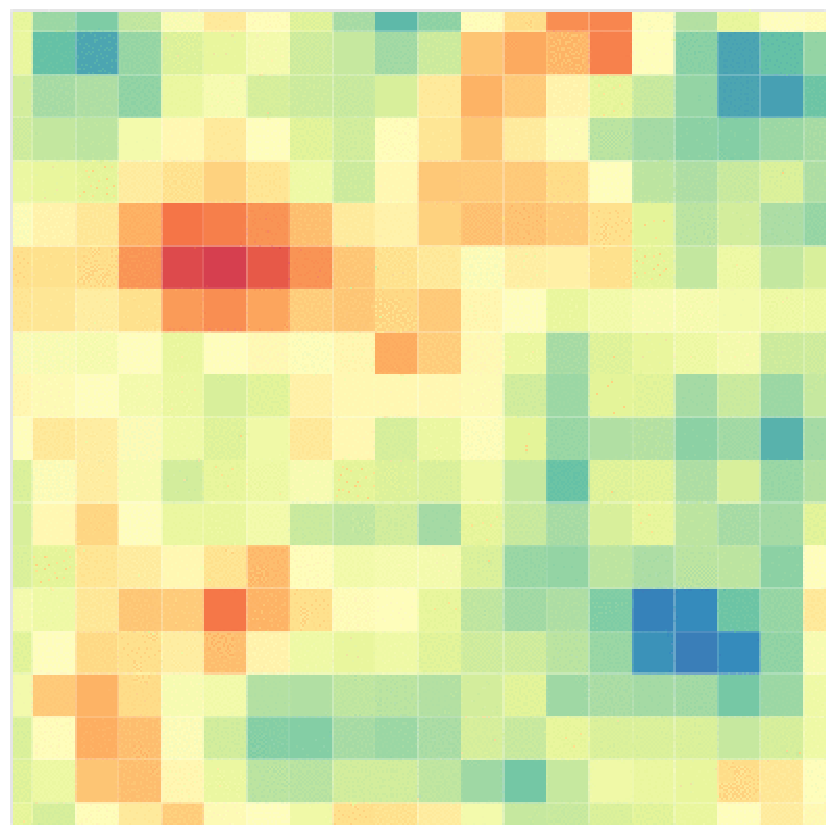
\includegraphics[width=0.28\linewidth]{Animations/animations/truth_5.pdf} & 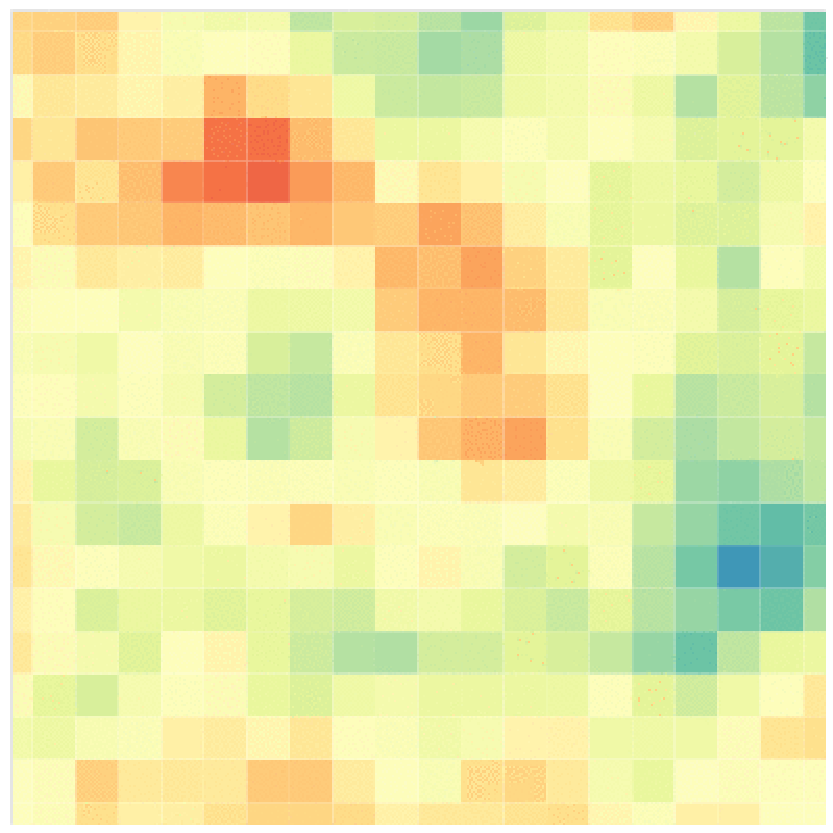
\includegraphics[width=0.28\linewidth]{Animations/animations/truth_15.pdf} & 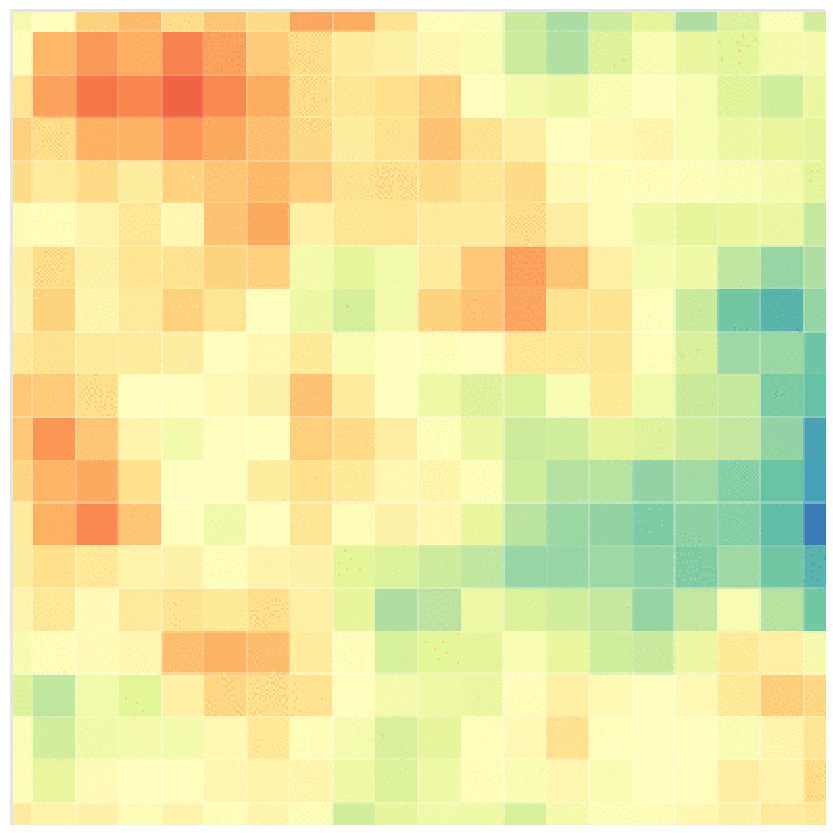
\includegraphics[width=0.28\linewidth]{Animations/animations/truth_25.pdf} \\ \pause
%		%\hline
%		$\textbf{y}_t$ & 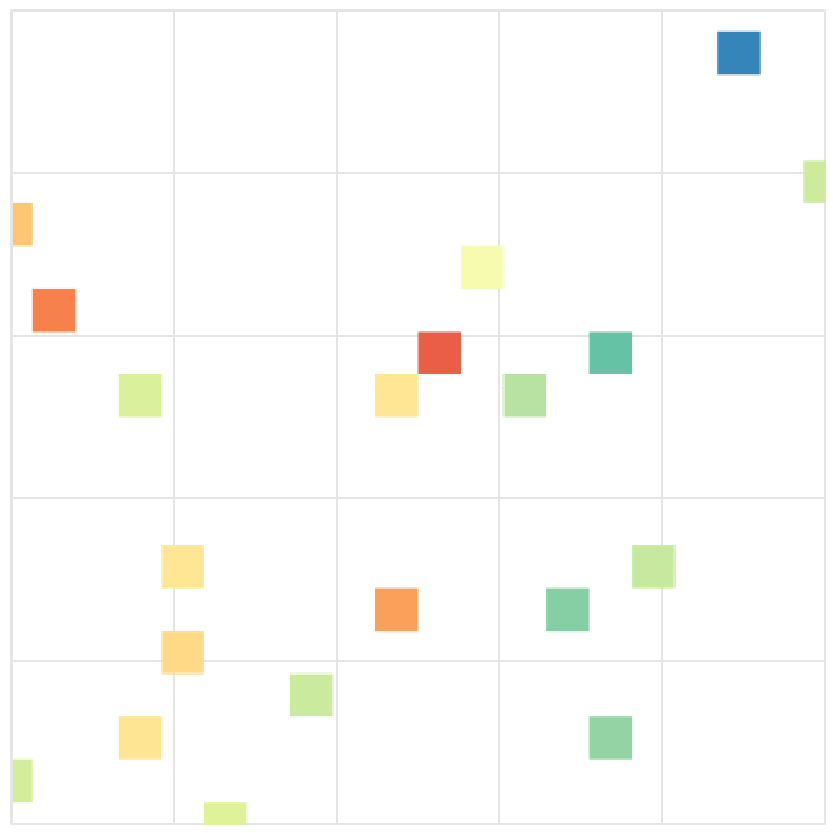
\includegraphics[width=0.28\linewidth]{Animations/animations/animate_5.pdf} & 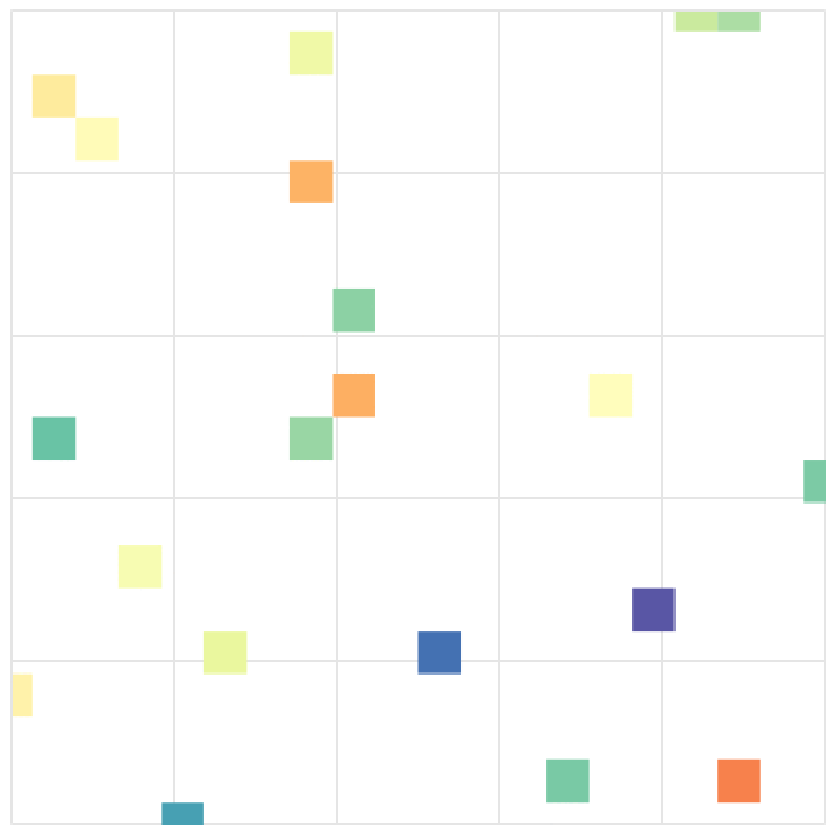
\includegraphics[width=0.28\linewidth]{Animations/animations/animate_15.pdf} & 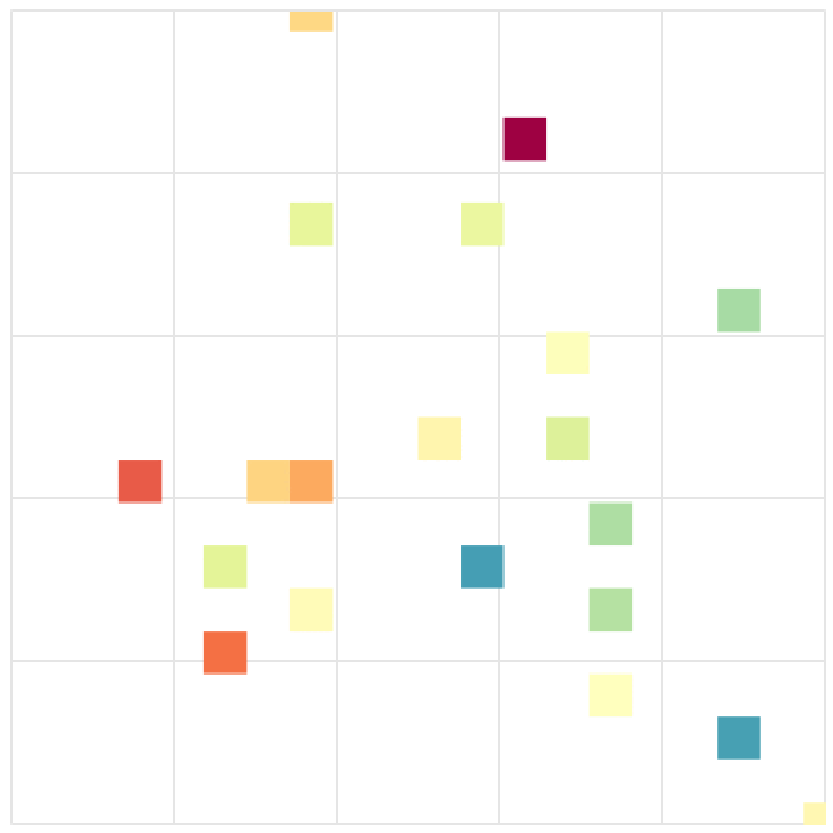
\includegraphics[width=0.28\linewidth]{Animations/animations/animate_25.pdf}
%	\end{tabular}
%\end{table}
%
%\end{frame}




\begin{frame}
	\frametitle{First step - spatial problem}
	Naive solution: conditional distributions
	
	Assume 
	\begin{align*}	
	\bx &\sim \normal(\bfmu, \bfSigma)\\ 
	\\
	\by &= \bH\bx + \bv, \quad \text{where} \quad \bv \sim \normal(\bfzero, \bR)
	\end{align*}\pause
	then	
	$$\bx | \by\sim \normal(\widetilde{\bfmu}, \widetilde{\bfSigma})$$\pause
	where 
	\begin{align*}
		{\color{red} \bfLambda^{-1}} &= {\color{red}\bH\bfSigma\bH^\top + \bR  }\\
		\widetilde{\bfmu} &= \bfmu +  \bfSigma\bH^\top {\color{red}\bfLambda} (\by - \bH\bfmu)\\
		\widetilde{\bfSigma} &= \bfSigma +  \bfSigma\bH^\top {\color{red}\bfLambda} \bH\bfSigma
	\end{align*}
	
\end{frame}




\begin{frame}
	\frametitle{The hierarchical Vecchia (HV)  approximation}
	\begin{figure}[!htbp]
	\centering
		\begin{subfigure}{.99\textwidth}
			\centering
			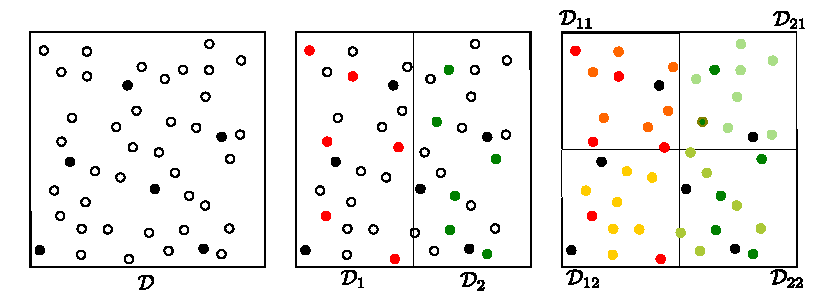
\includegraphics[trim=0 0 0 0, clip, width=0.75\textwidth]{images/domain.pdf}
			%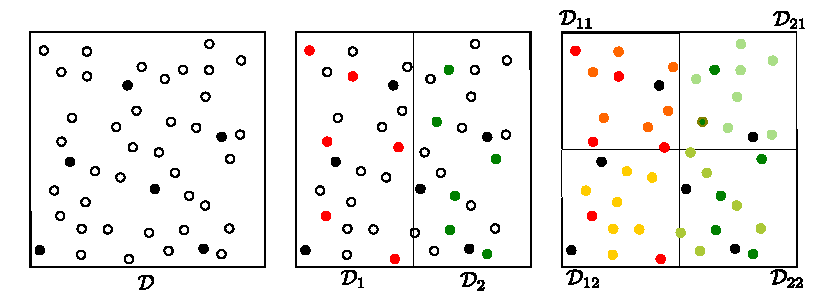
\includegraphics[trim=0 14 0 14, clip, width=0.75\textwidth]{images/domain.pdf}
		\end{subfigure}\\
	\end{figure}
    	\pause
	\begin{tabular}{rc}  
		\begin{tabular}{r}
		 \parbox{0.3\linewidth}{%  change the parbox width as appropiate
			$$\bx = \left[ \begin{array}{c} \sx\\ \sx_1\\ \sx_2\\ \sx_{11}\\ \sx_{12}\\ \sx_{21}\\ \sx_{22} \end{array}\right]$$
		}
           		\end{tabular} \pause
	      	& \begin{tabular}{c}
	            	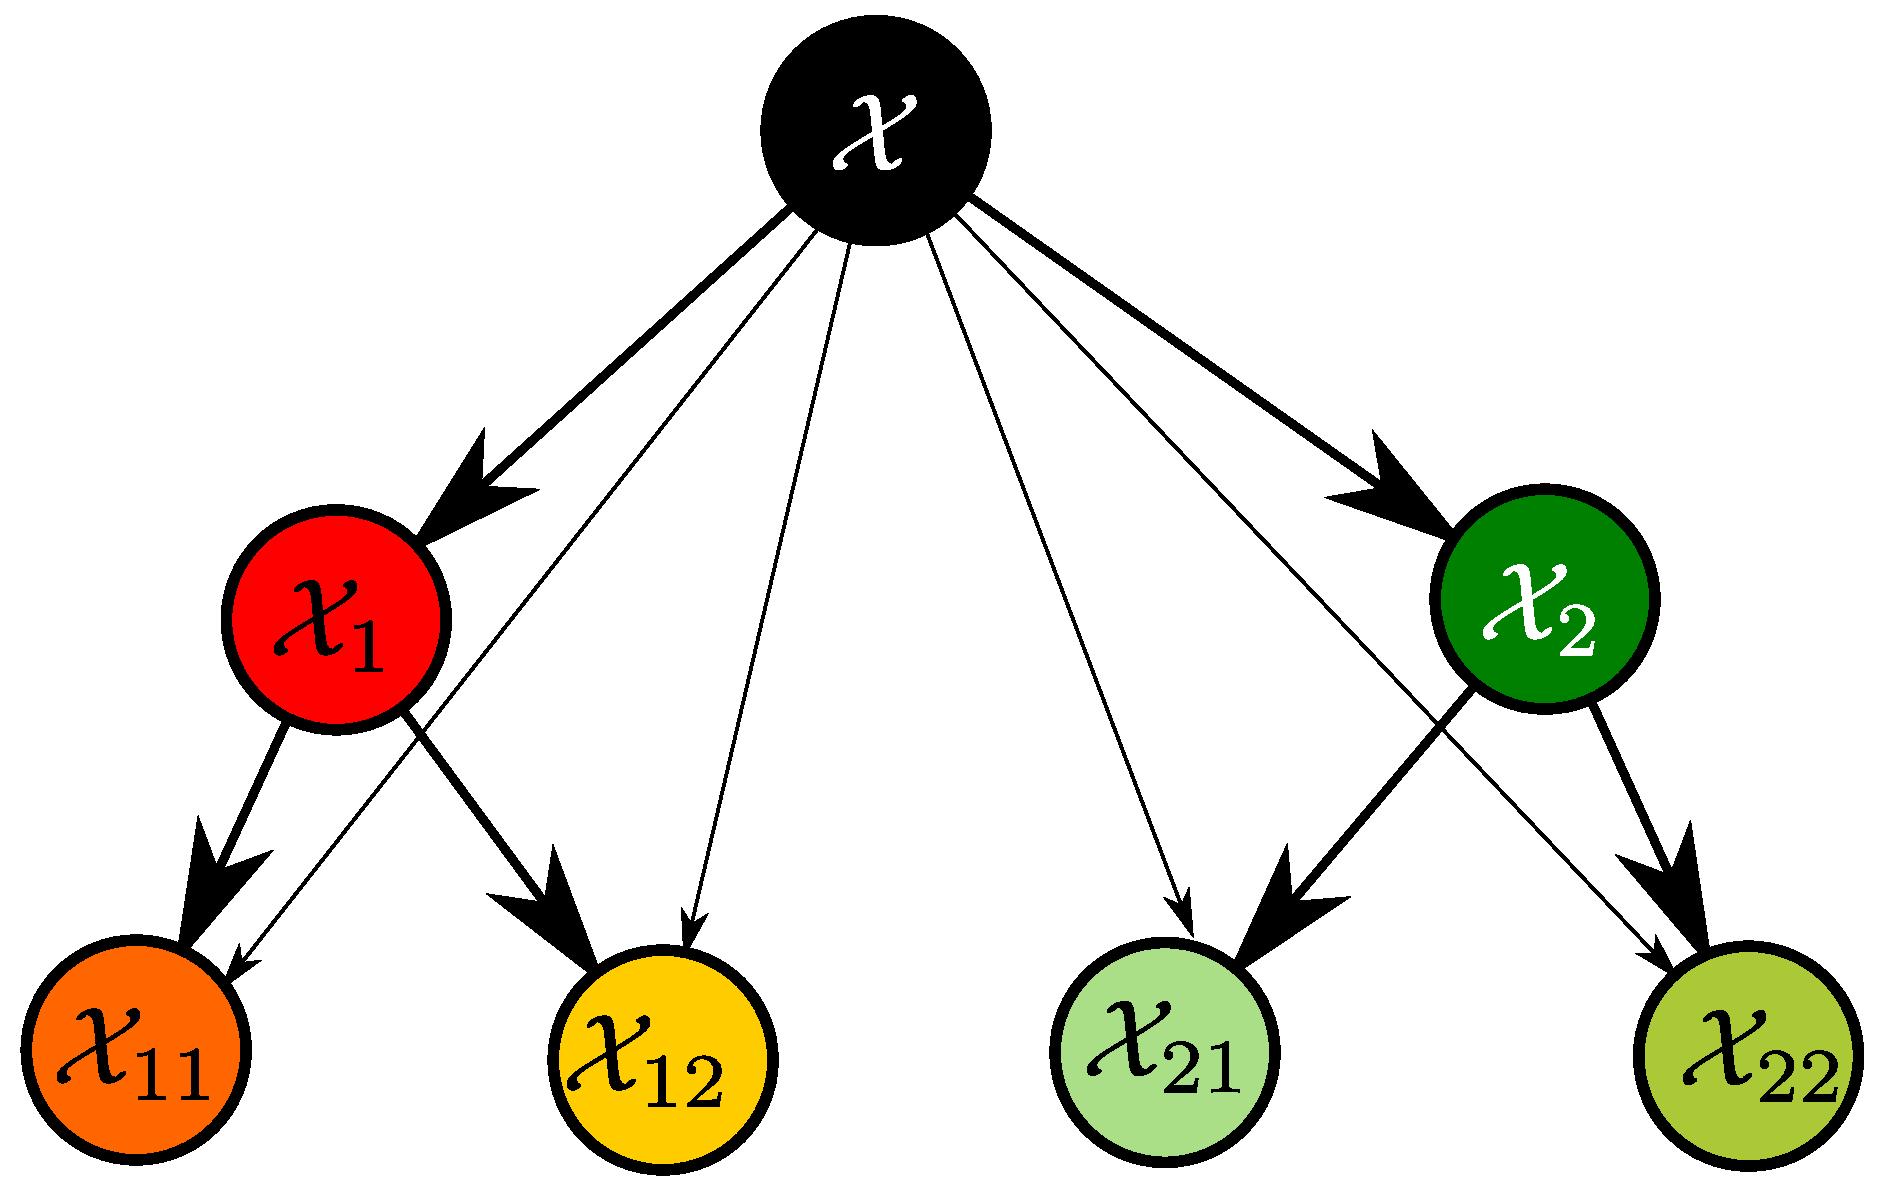
\includegraphics[scale=0.2]{images/graph.pdf}
		\end{tabular}  \\
	\end{tabular}
\end{frame}




\begin{frame}
	\frametitle{Incomplete Cholesky decomposition}
	\begin{algorithm}[H]
		\KwInput{ positive-definite matrix $\bA \in \mathbb{R}^{n \times n}$, sparsity matrix $\bS \in \{0,1\}^{n \times n}$}
		\KwResult{ lower-triangular $n\times n$ matrix $\bL$ }
		\begin{algorithmic}[1]
			\FOR{$i=1$ to $n$}
			\FOR{$j=1$ to $i-1$}
			\IF{$\bS_{i,j}=1$}
			\STATE $\bL_{i,j} = \frac{1}{\bL_{j,j}}\left(\bA_{i,j} - \sum_{k=1}^{j-1}\bL_{i,k}\bL_{j,k}\right)$ \\
			\ENDIF
			\ENDFOR 
			\STATE $\bL_{i,i} = \sqrt{\bA_{i,i} - \sum_{k=1}^{i-1}\bL_{k,k}}$
			\ENDFOR
		\end{algorithmic}
	\end{algorithm}
\end{frame}



\begin{frame}
	\frametitle{back to the HV approximation}
	
	\begin{tabular}{cc}
	The graph & corresponding $\bS$ \\
	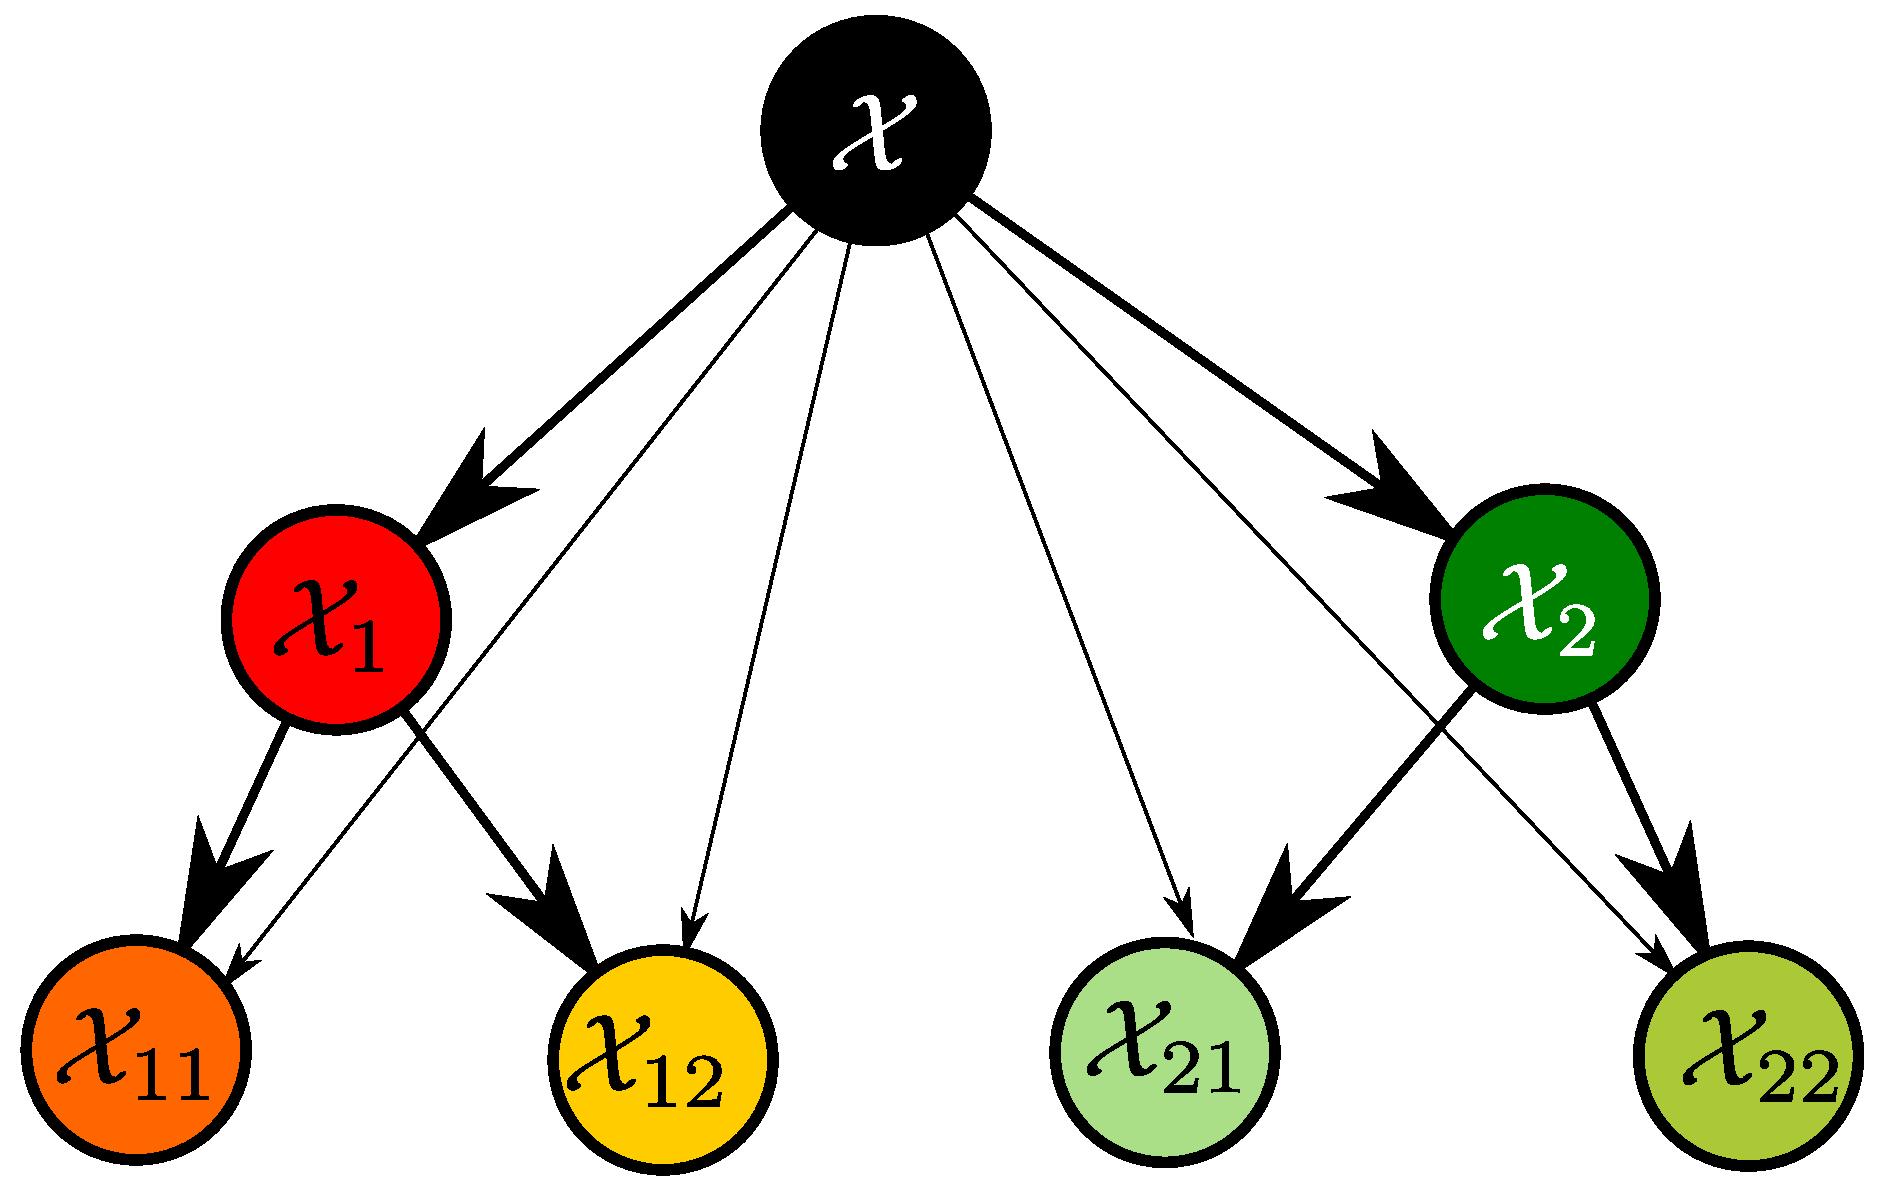
\includegraphics[scale=0.2]{images/graph.pdf} & 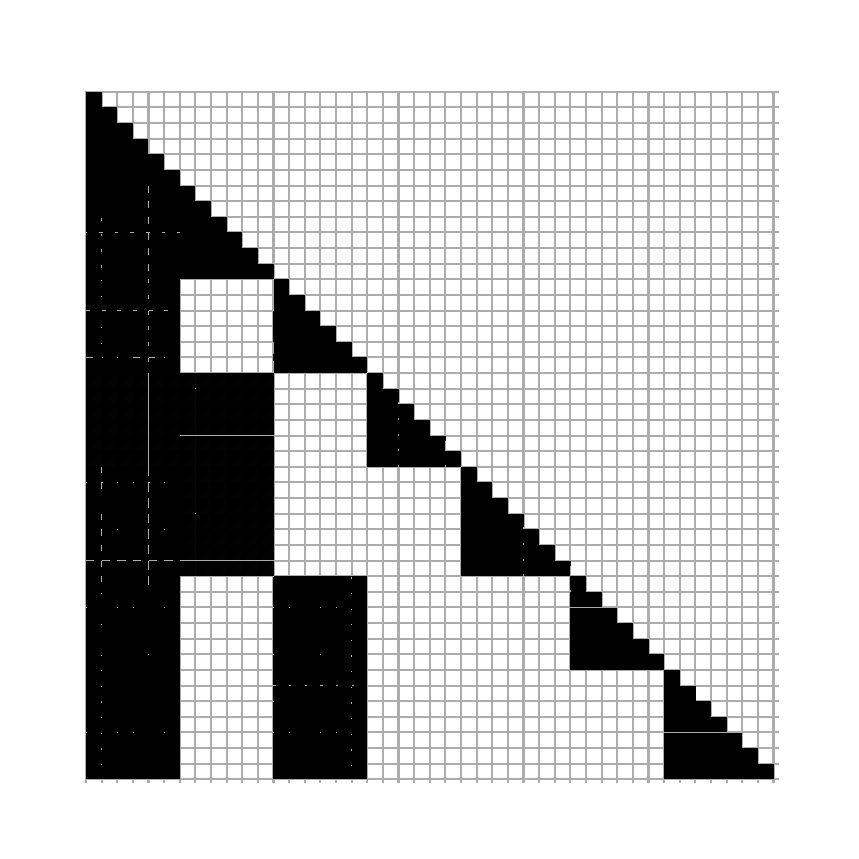
\includegraphics[scale=0.3]{images/S.pdf} 
	\end{tabular}
	
\end{frame}


\begin{frame}
\frametitle{Sparsity patterns (we proved it)}
		\begin{figure}
			\centering
			\begin{tabular}{cc}
			\raisebox{-.5\height}{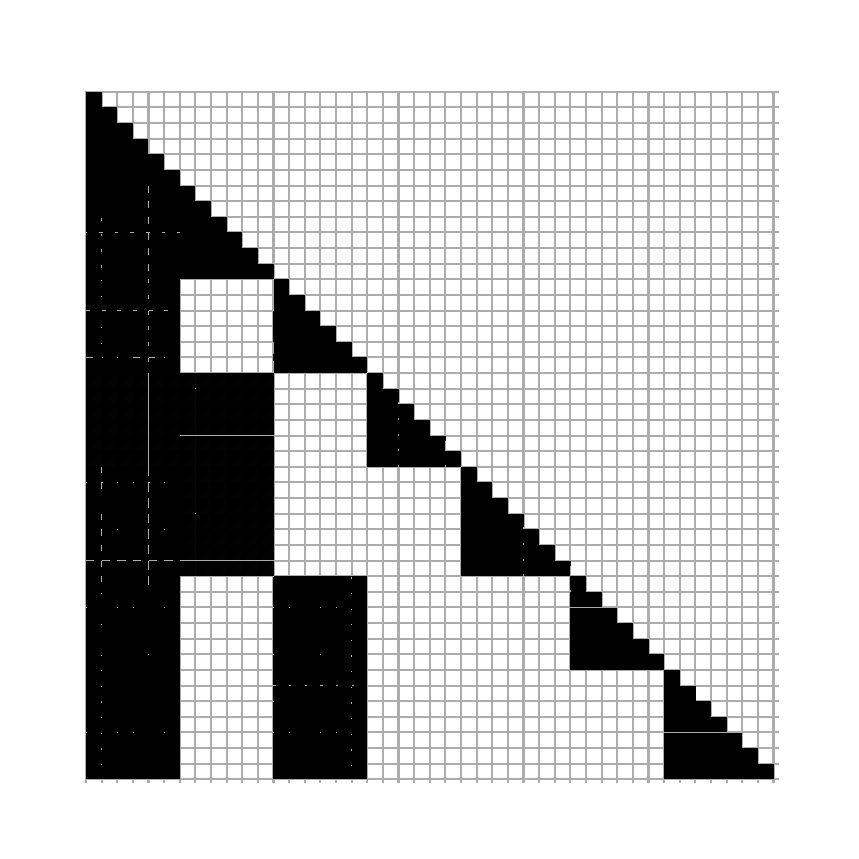
\includegraphics[scale=0.22]{images/S.pdf}} &  \raisebox{-.5\height}{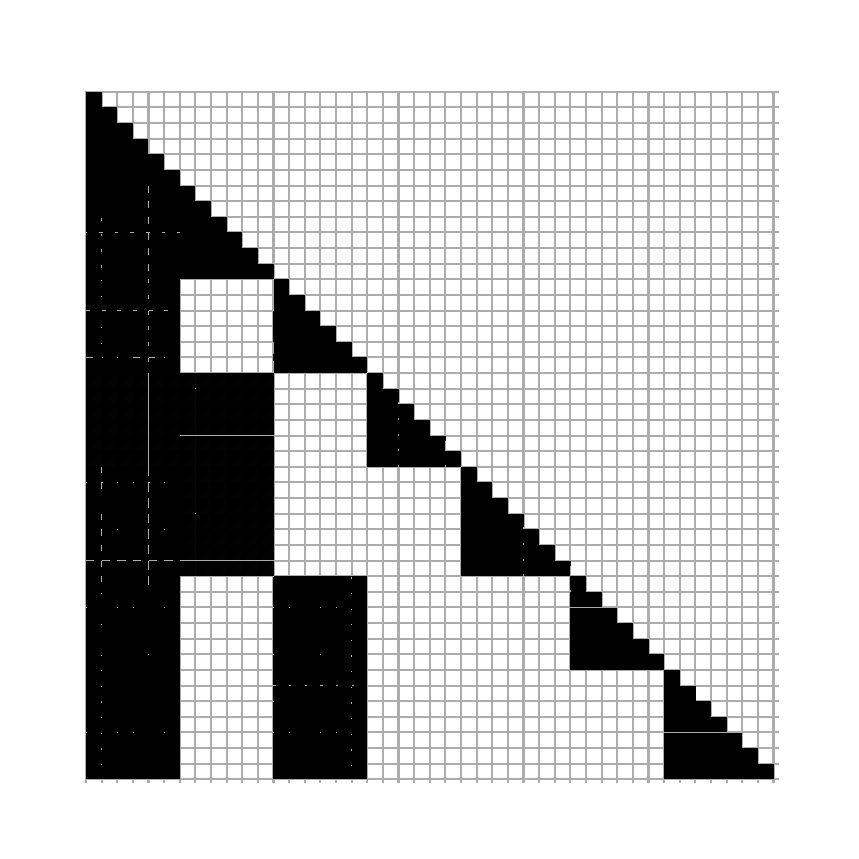
\includegraphics[scale=0.22]{images/S.pdf}}  \\
			$\bS$ & $\bL \colonequals \ichol(\bfSigma, \bS)$ \\
			\raisebox{-.5\height}{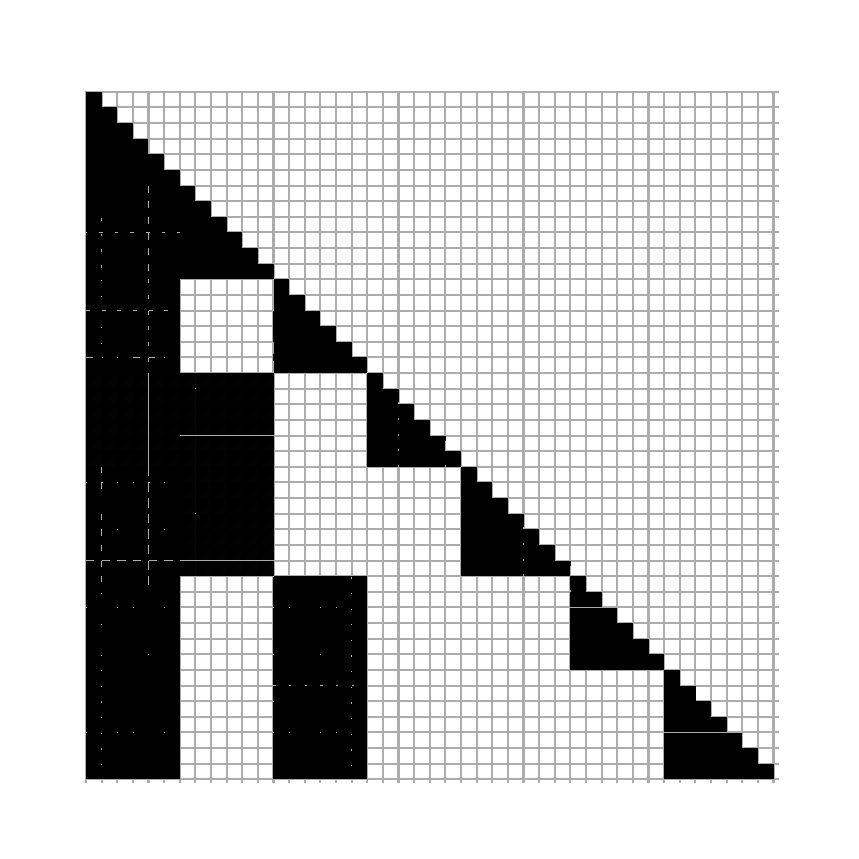
\includegraphics[scale=0.22]{images/S.pdf}} &  \raisebox{-.5\height}{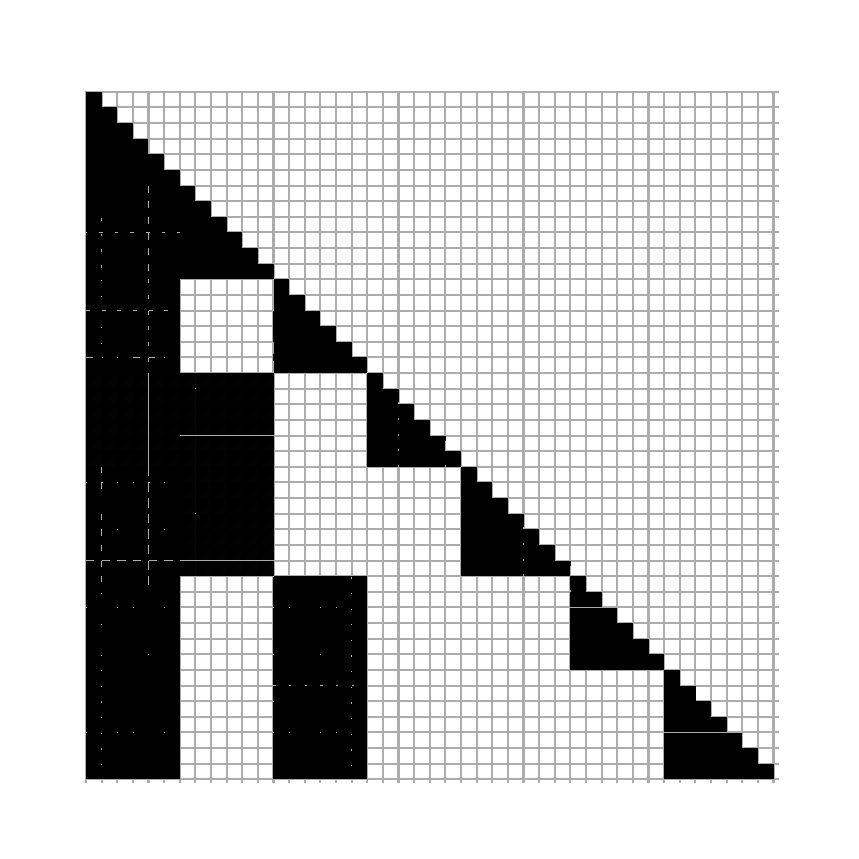
\includegraphics[scale=0.22]{images/S.pdf}}  \\
			$\bL^{-1}$ & $\widetilde{\bL} \colonequals \left( \bP\chol(\bP\bfLambda\bP)\bP\right)^{-\top}$  \\
			\end{tabular}
		\end{figure}
\end{frame}



\begin{frame}
	\frametitle{Some matrix algebra}
	The goal:
	\begin{align*}
		\widetilde{\bfmu} &= \bfmu +  \bfSigma\bH^\top {\color{red}\bfLambda} (\by - \bH\bfmu)\\
		\widetilde{\bfSigma} &= \bfSigma +  \bfSigma\bH^\top {\color{red}\bfLambda} \bH\bfSigma
	\end{align*}
	where ${\color{red} \bfLambda^{-1}} = \bH\bfSigma\bH^\top + \bR$.\pause
	\begin{align*}
	& &\bfSigma \approx \bL\bL^\top \quad &\implies &{\color{red}\bfLambda} &\approx \bL^{-\top}\bL^{-1} + \bH^\top\bR^{-1}\bH\\
	& &\left.\begin{array}{c} \bP\text{ - reverses order}\\ \widetilde{\bL} = \left( \bP\chol(\bP\bfLambda\bP)\bP\right)^{-\top} \end{array} \right\}  & \implies &\widetilde{\bfSigma} & \approx \widetilde{\bL} \widetilde{\bL}^\top\\
	& & & &\widetilde{\bfmu} &\approx \bfmu +\widetilde{\bL}\widetilde{\bL}^{-\top}\bH^{\top}\bR^{-1}\left(\by - \bH \bfmu\right)
	\end{align*}
\end{frame}



\begin{frame}
	\frametitle{Posterior inference using HV}	
	\begin{algorithm}[H]
		\KwInput{$\by, \bS, \bfmu, \bfSigma, \bH, \bR$}
		\vspace{0.3cm}
		\KwResult{$\widetilde\bfmu$ and $\widetilde\bL$}
		\vspace{0.3cm}
		\begin{algorithmic}[1]
			\STATE $\bL = \ichol(\bfSigma, \bS)$
			\vspace{0.1cm}
			\STATE $\bU = \bL^{-\top}$
			\vspace{0.1cm}
			\STATE $\bfLambda = \bU\bU^\top + \bH^\top\bR^{-1}\bH$
			\vspace{0.1cm}
			\STATE $\widetilde{\bL} = (\bP\left(\chol(\bP\bfLambda\bP)\right)\bP)^{-\top}$, where $\bP$ is the order-reversing permutation matrix
			\vspace{0.1cm}
			\STATE $\widetilde{\bfmu} = \bfmu + \widetilde{\bL}\widetilde{\bL}^\top\bH^{\top}\bR^{-1}\left(\by - \bH \bfmu\right)$
		\end{algorithmic}
		\label{alg:VF}
	\end{algorithm}
	\vfill\pause
	Can be easily extended to non-Gaussian data using the Vecchia-Laplace algorithm (Zilber \& Katzfuss, 2019)
\end{frame}




\begin{frame}
	\frametitle{Adding time}
	Assume that 
	$$
	\bx_t = \mathcal{E}_t(\bx_{t-1}) + \bw_t, \quad \quad \bw_t \sim \normal(\bfzero, \bQ_t)
	$$
	At each time $t$ we want to know the \emph{filtering distribution}:
	$$
	\bx_t | \by_{1:t} \sim \normal(\bfmu_{t|t}, \bfSigma_{t|t})
	$$
	which is Gaussian, provided that $\bx_0 | \by_0$ is Gaussian.
\end{frame}





\begin{frame}
	\frametitle{Extended Kalman filter}
	\textbf{Idea}: recursion
	\begin{itemize}
		\item Want $\bx_t|\by_{1:t}$
		\item Assume we know $\bx_{t-1}|\by_{1:t-1} \sim \normal(\bfmu_{t-1|t-1}, \bfSigma_{t-1|t-1})$
	\end{itemize}
	\vfill
	\textbf{Best guess (\emph{forecast})}: \\
	\vfill
	\begin{tabular}{rcccl}
		$\mathbb{E}(\bx_t| \by_{t-1})$ & $\colonequals$ & $\bfmu_{t|t-1}$  & $=$ & $\evol_t(\bfmu_{t-1|t-1})$ \\
		\\
		$\levol_t$ & $\colonequals$ & $\nabla \evol_t(\bfmu_{t-1|t-1})$ & & \\
		$\var(\bx_t | \by_{t-1})$ & $\colonequals$ & $\bfSigma_{t|t-1}$ & $=$ & $\bE_t \bfSigma_{t-1|t-1} \bE_t^{\top} + \bQ_t$\\
	\end{tabular}
	
	\vspace{1cm}
	\textbf{\emph{Update} current data ($\by_t$)}\\
			(posterior inference using $\bfmu_{t|t-1}$ and $\bfSigma_{t|t-1}$ as prior moments)
\end{frame}



\begin{frame}
	\frametitle{Extended Kalman-Vecchia filter}
	\begin{algorithm}[H]
		\KwInput{$\bS$, $\bfmu_{0|0}$, $\bfSigma_{0|0}$, $\{(\by_t,\evol_t,\bQ_t, \bH_t, \bR_t) \}_{ t=1,2,\ldots}$,}
		\vspace{0.3cm}
		\KwResult{$\bfmu_{t|t}$ and $\bL_{t|t}$}%, such that $\hat{p}(\bx_t|\by_{1:t}) = \normal_n(\bx_t|\bfmu_{t|t},\bL_{t|t}\bL_{t|t}^\top)$}
		\vspace{0.3cm}
		\begin{algorithmic}[1]
			\STATE Compute $\bL_{0|0} = \left( \ichol(\bfSigma_{0|0}, \bS\right))^{-\top}$% and $\bL_{0|0} = \bU_{0|0}^{-\top}$
			\vspace{0.1cm}
			\FOR{$t = 1, 2, \dots$}
				\vspace{0.1cm}
	    			\STATE Calculate $\levol_t = \nabla\evol_t(\bfmu_{t-1|t-1})$%\frac{\partial \evol_t(\bx_{t-1})}{\partial \bx_{t-1}} \big|_{\bx_{t-1} = \bfmu_{t-1|t-1} }$ \label{ln:jacobian}
				\vspace{0.2cm}
			    	\STATE Forecast: $\begin{array}{c}\bfmu_{t|t-1} = \evol_t(\bfmu_{t-1|t-1})\\ \bL_{t|t-1} = \levol_t\bL_{t-1|t-1}\end{array}$
				\vspace{0.2cm}
			     	\STATE Calculate $\bfSigma_{t|t-1; i,j} = \bL_{t|t-1;i,:} \bL_{t|t-1;j,:}^\top + \bQ_{t;i,j}$ ($i,j:\;,\bS_{i,j}=1)$:
				\vspace{0.1cm}
				\STATE Update: $[\bfmu_t, \bL_{t|t}] = \text{HV}(\by_t, \bS, \bfmu_{t|t-1}, \bfSigma_{t|t-1}, \bH_t, \bR_t$)
				\vspace{0.1cm}
				\RETURN $\bfmu_{t|t}, \bL_{t|t}$
			\ENDFOR
		\end{algorithmic}
	\label{alg:eKVLfilter}
	\end{algorithm}
\end{frame}



\begin{frame}
\begin{figure}
	\begin{subfigure}{1.0\textwidth}
%		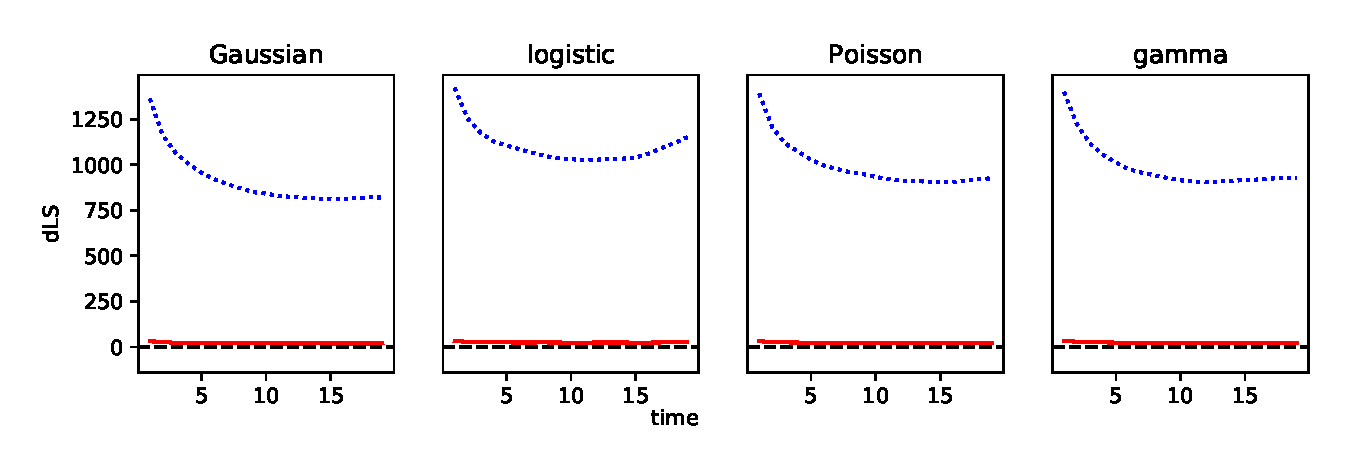
\includegraphics[trim={0, 3mm, 0, 0}, clip, width=1.0\textwidth]{images/lorenz-dLS.pdf}
		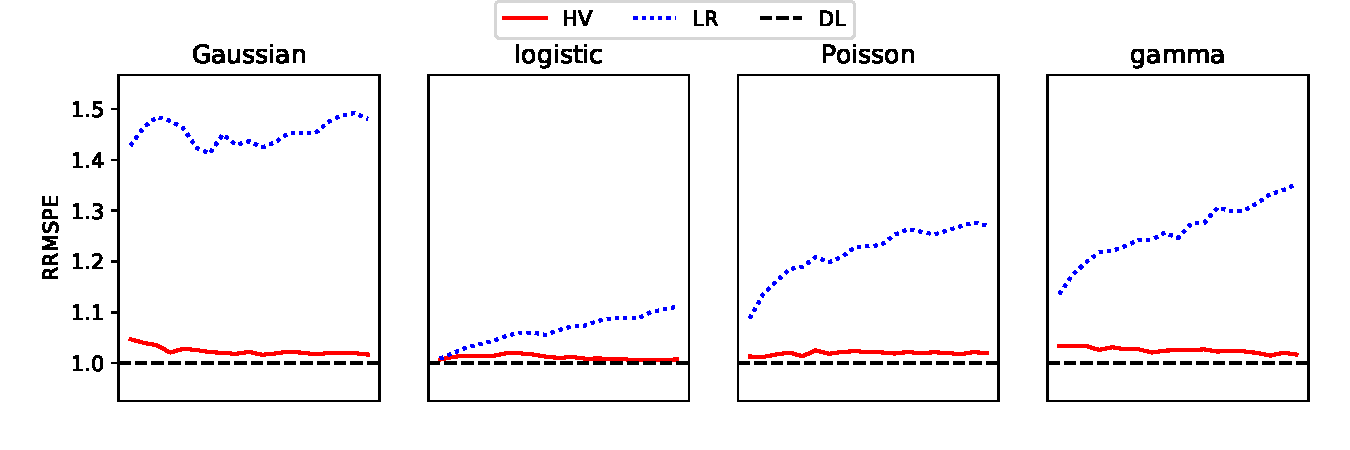
\includegraphics[width=1.0\textwidth]{images/lorenz-RRMSPE.pdf}
	\end{subfigure}
	\begin{subfigure}{1.0\textwidth}
%		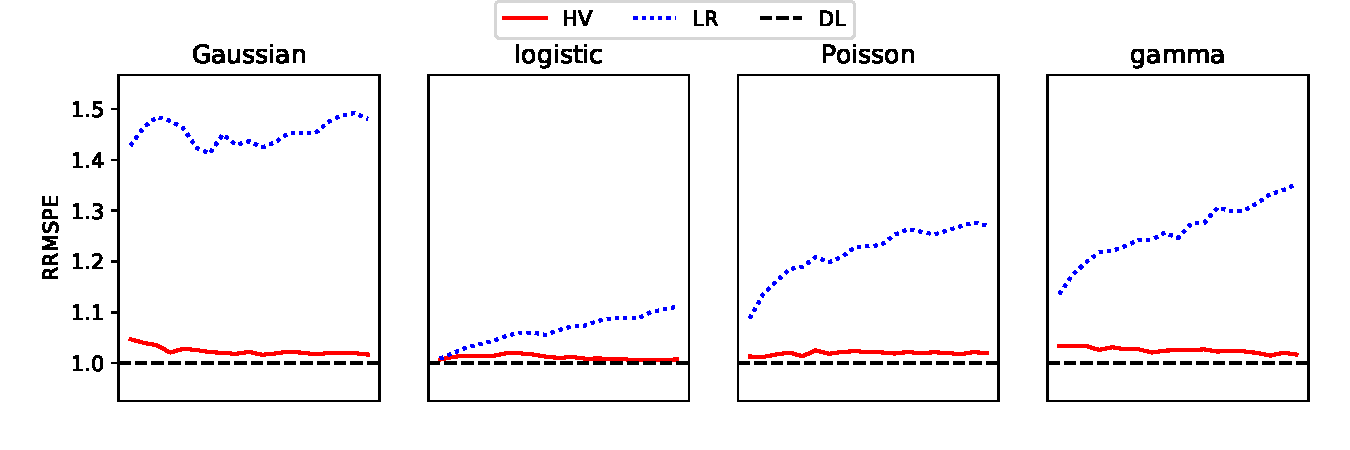
\includegraphics[trim={0, 3mm, 0, 5mm}, clip, width=1.0\textwidth]{images/lorenz-RRMSPE.pdf}
		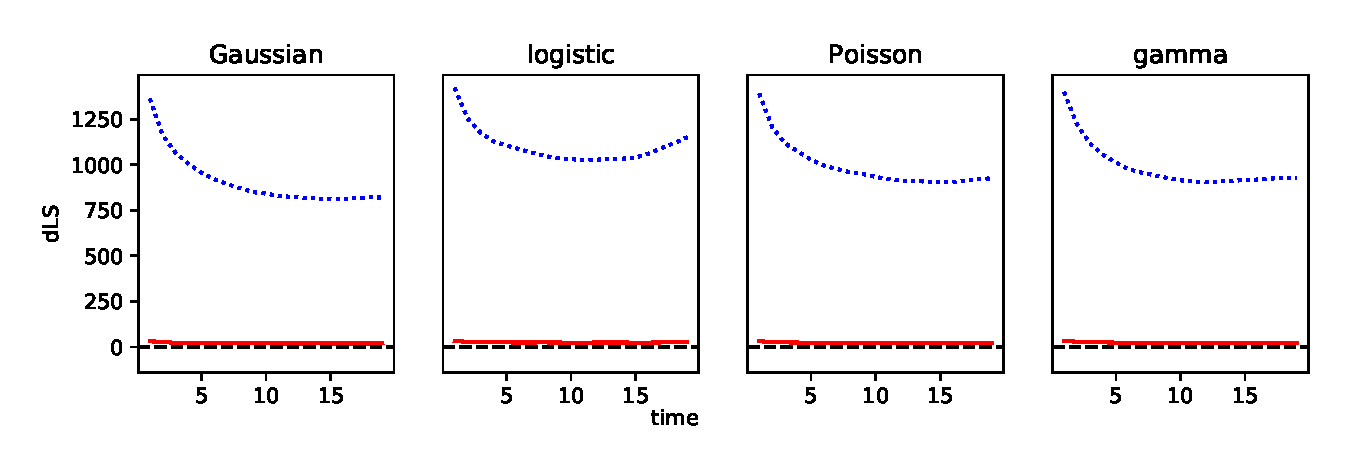
\includegraphics[width=1.0\textwidth]{images/lorenz-dLS.pdf}
	\end{subfigure}
%	\begin{subfigure}{1.0\textwidth}
%		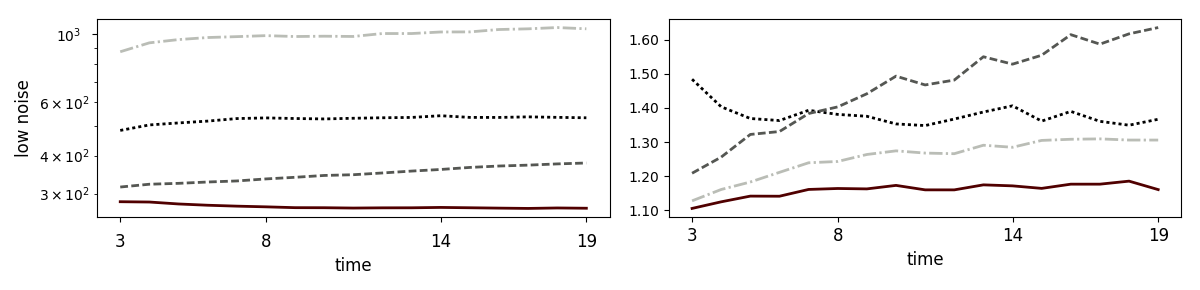
\includegraphics[trim={0, 4mm, 0, 5mm}, clip, width=1.0\textwidth]{images/strong_signal2d.png}
%	\end{subfigure}
	\vspace{-1mm}
	\label{fig:scores-2d}
\end{figure} 
\end{frame}



%\begin{frame}
%	\frametitle{Illustration}
%	\begin{tabular}{c}
%		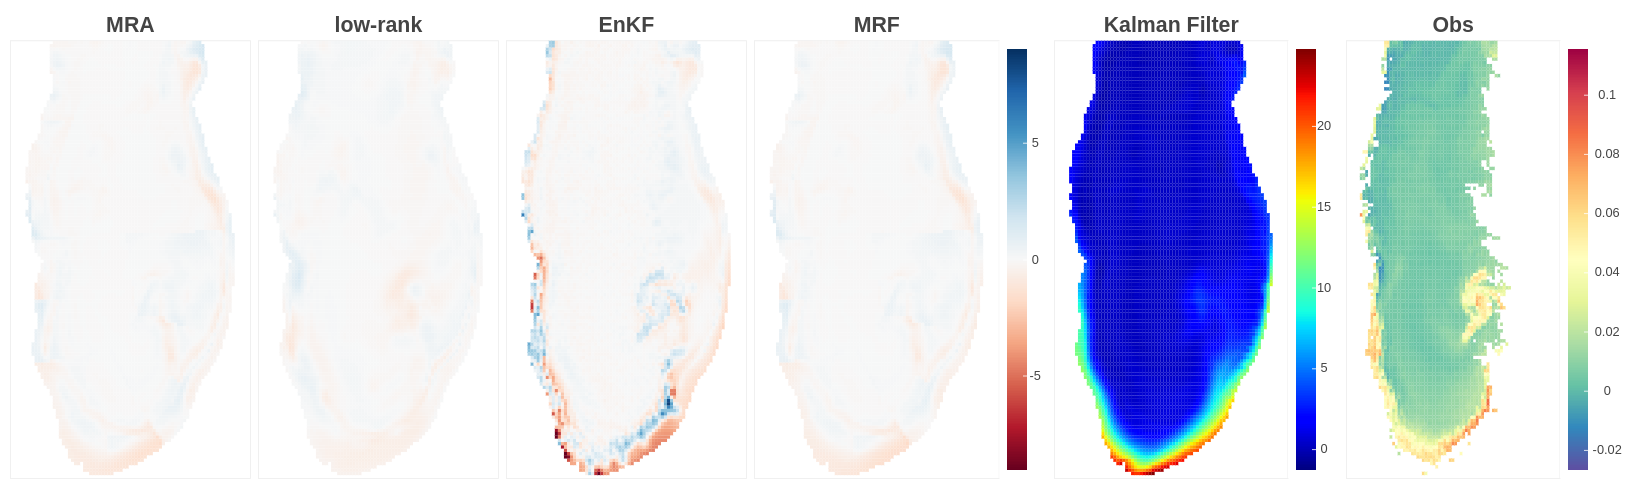
\includegraphics[trim=200 0 0 0, clip, width=1.0\textwidth]{images/282.png}\\
%		\\
%		$t=2$
%	\end{tabular}
%\end{frame}
%\begin{frame}
%	\frametitle{Illustration}
%	\begin{tabular}{c}
%		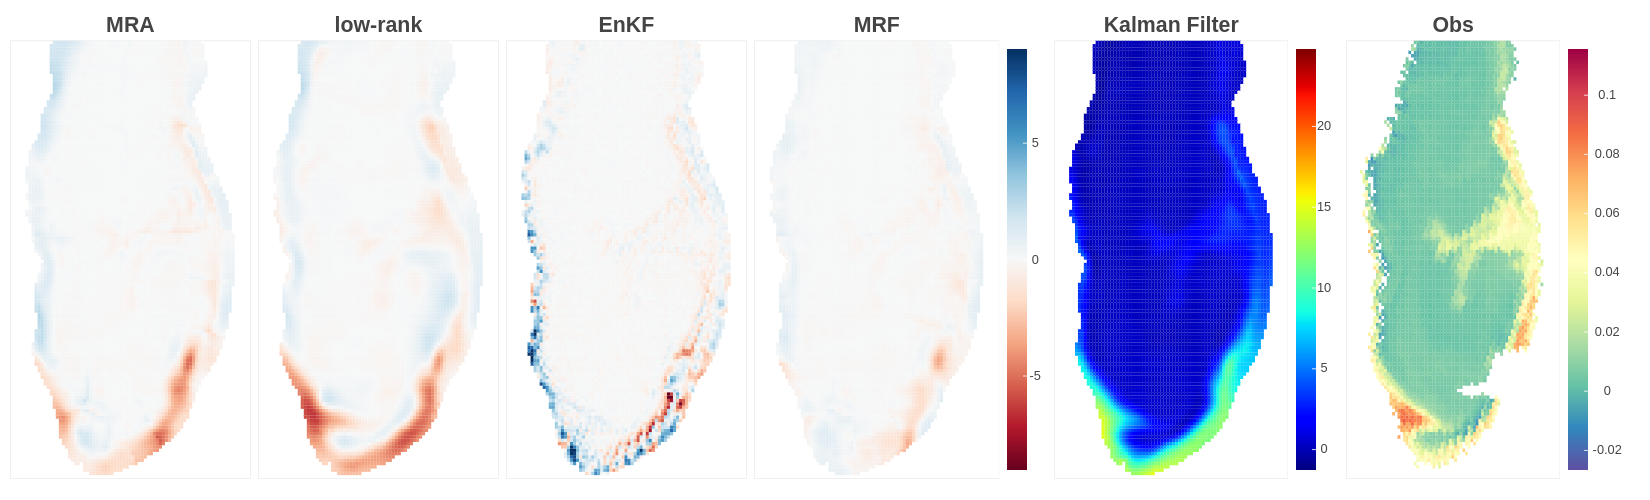
\includegraphics[trim=200 0 0 0, clip, width=1.0\textwidth]{images/547.png}\\
%		\\
%		$t=267$
%	\end{tabular}
%\end{frame}
%\begin{frame}
%	\frametitle{Illustration}
%	\begin{tabular}{c}
%		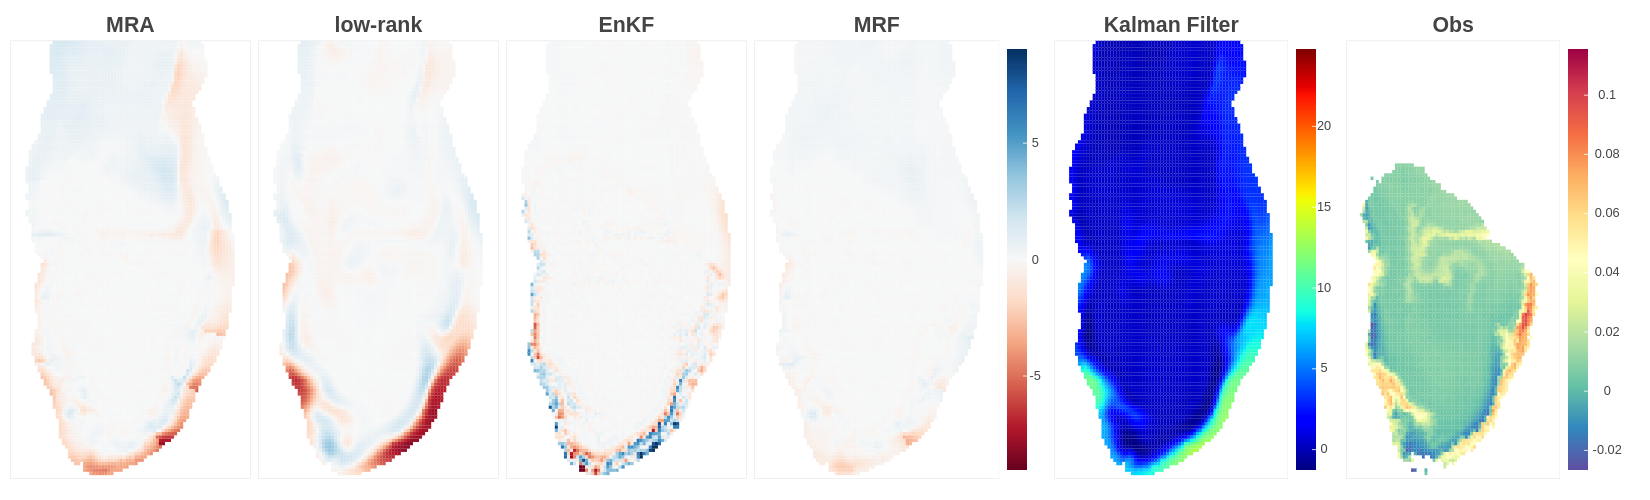
\includegraphics[trim=200 0 0 0, clip, width=1.0\textwidth]{images/689.png}\\
%		\\
%		$t=409$
%	\end{tabular}
%\end{frame}


\begin{frame}
\centering
\huge{Thanks!}

\vspace{1cm}
\centering
\Large{\url{https://arxiv.org/pdf/2006.16901.pdf}}
\end{frame}

%	\centering
%	\begin{tabular}{c}
% \\
%		 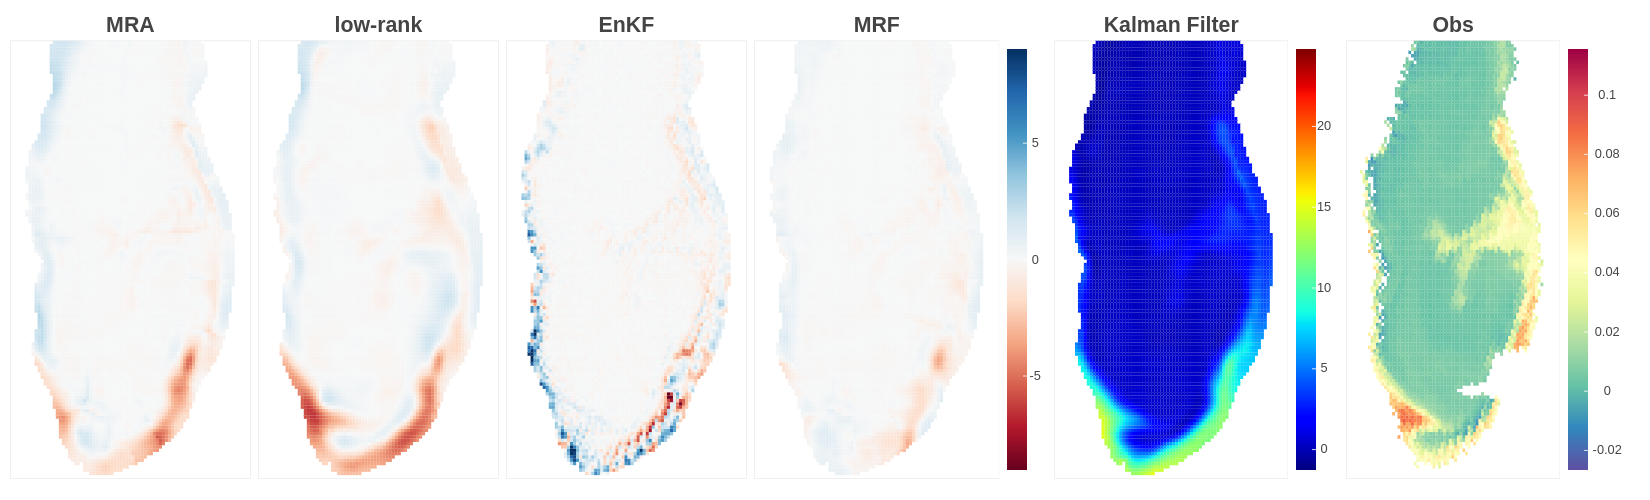
\includegraphics[angle=0,origin=c,width=0.81\textwidth]{images/547.png} \\
%		  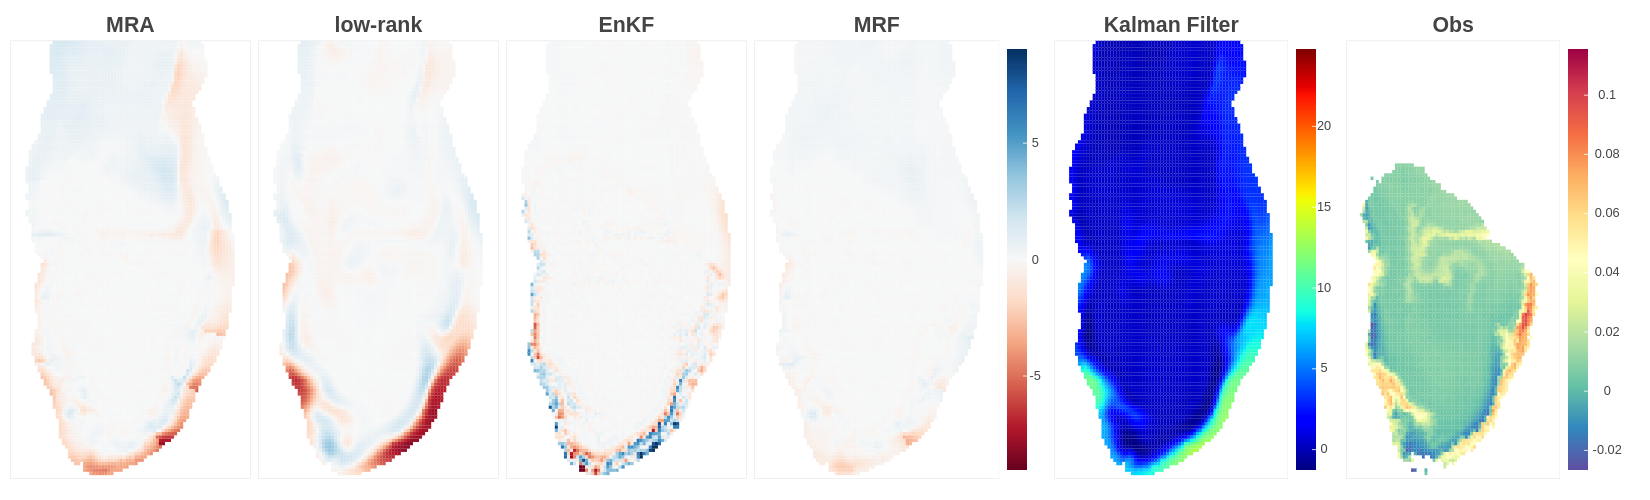
\includegraphics[angle=0,origin=c,width=0.81\textwidth]{images/689.png} \\

	%\small	(a) t = 2 & (b) t= 267 & (c) t=409
	%\vspace{1mm}	
%	\end{tabular}
	%\caption{Satellite data (in log RSR) and exact Kalman filtering means of sediment concentrations (in mg/L), along with differences of approximate filtering means to the Kalman filter. We display the results for the southern basin of the lake only, where differences between the methods are most pronounced.}
%\end{figure}
%\end{frame}


\end{document}
%-------------------------------------------------------------------------------------------------



